\phantomsection

\chapter{Pre-Exploitation}
\markboth{Pre-Exploitation}{}

\section{Target Scoping} { \setstretch{1.3}}
Il processo di \emph{Penetration Testing}, come evidenziato nella fase introduttiva, ha uno scopo puramente didattico, per cui non è prevista una fase di accordo tra le parti coinvolte in quanto l'asset da analizzare è una macchina virtuale vulnerabile \emph{by design}. Non vi è, infatti, un cliente dal quale raccogliere requisiti e con il quale definire obiettivi di business e modelli dei costi. Il processo verrà svolto senza particolari vincoli formali relativi all'asset.

\section{Information Gathering} { \setstretch{1.3}}
La caratterizzazione dell'asset da analizzare può generalmente avvenire mediante molteplici \emph{tool} e coinvolgere diversi aspetti dell'asset stesso. Dal momento che si sta trattando una macchina virtuale vulnerabile \emph{by-design} contestualizzata in un'attività progettuale avente uno scopo didattico non risulta utile ricorrere a particolari tecniche \emph{OSINT (Open Source INTelligence)}, né a tecniche volte all'ottenimento di informazioni di routing e record DNS. Sono state, tuttavia, consultate le informazioni di base dell'asset disponibili sulla piattaforma \emph{VulnHub} che mette a disposizione la macchina virtuale. Le informazioni fornite sono le seguenti:
\begin{itemize}
    \item \textbf{Nome della macchina}: \emph{Momentum: 1};
    \item \textbf{Sistema Operativo}: \emph{Linux};
    \item \textbf{DHCP Server}: abilitato;
    \item \textbf{Indirizzo \emph{IP}}: assegnato in automatico.
\end{itemize}
Non risultano, dunque, note le informazioni relative all'indirizzo \emph{IP} della macchina né le credenziali di accesso alla stessa. 
\section{Target Discovery} { \setstretch{1.3}}
L'individuazione della macchina \emph{Momentum: 1} all'interno della rete è stata effettuata, in accordo con quanto descritto nel capitolo introduttivo, utilizzando una macchina virtuale con \emph{Kali Linux} connessa alla medesima rete. 
\subsection{Informazioni preliminari}
Prima di procedere alla trattazione delle metodologie di individuazione della macchina target è necessario considerare alcuni aspetti dell'architettura di rete virtuale nell'ambito della quale è stata svolta l'attività di \emph{Penetration Testing}. La gestione del \emph{NAT} e del \emph{DHCP} da parte di \emph{VirtualBox} fa sì che risultino connessi alla rete degli host aventi \emph{IP} \emph{10.0.2.1}, \emph{10.0.2.2} e \emph{10.0.2.3}. Alla rete risulterà altresì connessa la macchina virtuale con \emph{Kali Linux} della quale è stato rilevato l'indirizzo \emph{IP} (\emph{10.0.2.15}) mediante il comando \emph{ifconfig} il cui output è illustrato nella figura \ref{fig:ifconfig}. 
\begin{figure}[h]
    \centering
    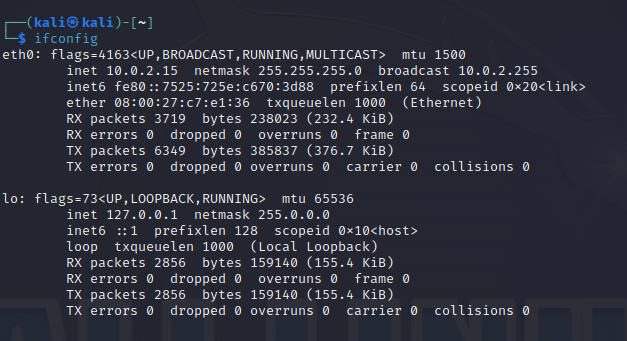
\includegraphics[scale=0.8]{capitoli/images/ifconfig.png}
    \caption{Output del comando \emph{ifconfig}}
    \label{fig:ifconfig}
\end{figure}
\subsection{Scansione con \emph{nmap}}
Come evidenziato in precedenza, l'indirizzo \emph{IP} di \emph{Momentum: 1} non è noto in quanto viene assegnato mediante il servizio di \emph{DHCP} di \emph{VirtualBox}. Per tale ragione è stata eseguita una scansione volta alla rilevazione della macchina target sulla rete \emph{10.0.2.0/24} mediante il comando:
\begin{lstlisting}[language=bash]
    $ nmap -sP 10.0.2.0/24
\end{lstlisting}
Questo comando effettua un \emph{ping scan} di tutti gli host della rete specificata in input \cite{nmap}, nell'ambito della quale vengono rilevati 3 host attivi, come mostrato nella figura \ref{fig:nmap}. Dal momento che, come specificato in precedenza, l'indirizzo \emph{10.0.2.1} fa riferimento ad un host di \emph{VirtualBox} e l'indirizzo \emph{10.0.2.15} è relativo alla macchina virtuale con \emph{Kali}, risulta immediato stabilire che l'indirizzo \emph{IP} di \emph{Momentum: 1} è \emph{10.0.2.4}.
\begin{figure}[h]
    \centering
    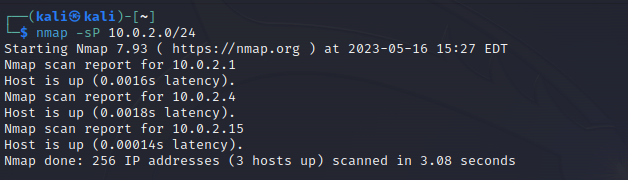
\includegraphics[scale=0.75]{capitoli/images/nmap.png}
    \caption{Output del comando \emph{nmap (ping scan)}}
    \label{fig:nmap}
\end{figure}
\subsection{Determinazione \emph{MAC Address} con \emph{arping}}
A partire dall'indirizzo \emph{IP} di \emph{Momentum: 1}, risulta possibile arricchire la conoscenza della macchina target individuandone il \emph{MAC Address}. Ciò è possibile mediante il comando:
\begin{lstlisting}[language=bash]
    $ sudo arping 10.0.2.4 -c 1
\end{lstlisting}
Tale comando invia un'\emph{ARP Request} al dispositivo indicato in input \cite{arping}. Mediante l'output, illustrato nella figura \ref{fig:arping}, si stabilisce che il \emph{MAC Address} di \emph{Momentum: 1} è \emph{08:00:27:0f:15:fd}.
\begin{figure}[h]
    \centering
    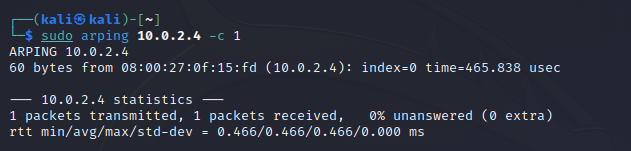
\includegraphics[scale=0.75]{capitoli/images/arping.png}
    \caption{Output del comando \emph{arping}}
    \label{fig:arping}
\end{figure}
\subsection{Scansione con \emph{arp-scan}}
Durante il processo di \emph{Penetration Testing} è stato utilizzato un approccio volto all'ottenimento delle medesime informazioni mediante molteplici tool al fine di confrontarne i risultati per massimizzare il quantitativo di informazioni ottenute nell'ambito di una determinata fase. A tale scopo ci si è serviti del tool \emph{arpscan} per effettuare una scansione sulla rete \emph{10.0.2.0/24} mediante il comando:
\begin{lstlisting}[language=bash]
    $ sudo arp-scan 10.0.2.0/24
\end{lstlisting}
\begin{figure}
    \centering
    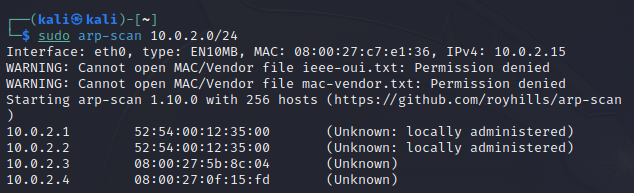
\includegraphics[scale=0.75]{capitoli/images/arpscan.png}
    \caption{Output del comando \emph{arp-scan}}
    \label{fig:arpscan}
\end{figure}
L'output del comando, illustrato nella figura \ref{fig:arpscan}, mostra che la scansione ha rilevato 4 host, per ciascuno dei quali ha fornito il relativo indirizzo \emph{IP} ed il relativo \emph{MAC Address}. La precedente scansione (effettuata con il tool \emph{nmap}) non ha rilevato gli host \emph{192.168.1.2} e \emph{192.168.1.3}, tuttavia, come evidenziato in precedenza, questi host sono gestiti da \emph{VirtualBox} per cui non hanno rilevanza nel processo di \emph{Penetration Testing} effettuato. L'host avente indirizzo \emph{IP} \emph{10.0.2.4} e \emph{MAC Address 08:00:27:0f:15:fd} è relativo alla macchina target.
\subsection{OS Fingerprinting attivo con \emph{nmap}}
Al fine di arricchire la conoscenza relativa alla macchina target è stata effettuata un'operazione di \emph{OS detection} mediante il comando:
\begin{lstlisting}[language=bash]
    $ sudo nmap -O 10.0.2.4
\end{lstlisting}
\begin{figure}
    \centering
    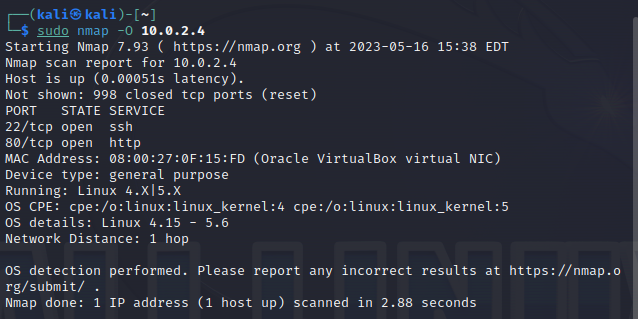
\includegraphics[scale=0.75]{capitoli/images/fingerprinting.png}
    \caption{Output del comando \emph{nmap (SO Fingerprinting)}}
    \label{fig:fingerprinting}
\end{figure}
L'output ottenuto (figura \ref{fig:fingerprinting}) fornisce diverse informazioni relative al sistema operativo in esecuzione sulla macchina target. È possibile stabilire che si tratta di un sistema \emph{Linux} presumibilmente ad una versione \emph{4.15} o \emph{5.6} (quando \emph{nmap} non riesce a stabilirlo con precisione mostra tutte i possibili match \cite{nmap-manual}); il tool fornisce, infine, la \emph{CPE} \footnote{\emph{CPE (Common Platform Enumeration)} è un sistema di naming strutturato per sistemi operativi, software e packages \cite{cpe}} di riferimento (\emph{cpe:/o:linux:linux\_kernel:4 cpe:/o:linux\_kernel:5}). Sono, altresì, presenti informazioni relative alle porte aperte ed ai servizi attivi sulla macchina target, che nell'ambito della fase di \emph{Target Discovery}, sono state sfruttate unicamente per effettuare OS Fingerprinting passivo; sulla macchina target risultano aperte la porta 80 (servizio \emph{HTTP}) e la porta 22 (servizio \emph{SSH}).
\subsection{OS Fingerprinting passivo con \emph{p0f}}
La fase di OS Fingerprinting attivo non ha portato all'individuazione dell'esatta versione del sistema operativo in esecuzione sulla macchina target: è stata, dunque, svolta una fase di OS Fingerprinting passivo finalizzata all'ottenimento di ulteriori informazioni in merito, utilizzando il tool \emph{p0f}. La tecnica di fingerprinting passivo adottata consiste nel porsi in ascolto su una specifica interfaccia di rete ed ispezionare i pacchetti \emph{TCP/IP} intercettati al fine di individuare le informazioni desiderate. Tale operazione è stata svolta mediante il comando (figura \ref{fig:p0f}):
\begin{lstlisting}[language=bash] 
    $ sudo p0f -i eth0 
\end{lstlisting}
\begin{figure}[h]
    \centering
    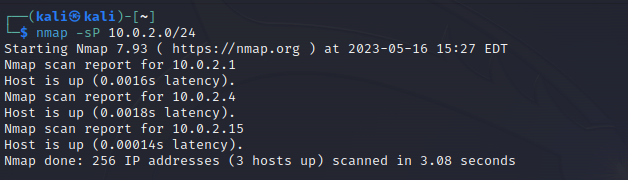
\includegraphics[scale=0.8]{capitoli/images/nmap.png}
    \caption{Output del comando \emph{p0f}}
    \label{fig:p0f}
\end{figure}
Il passo successivo consiste nel fare in modo che la macchina target invii pacchetti sull'interfaccia di rete \emph{eth0}; a tale scopo sono state effettuate delle richieste ai servizi esposti dalla macchina, ossia \emph{HTTP} e \emph{SSH}, mediante i comandi:
\begin{lstlisting}[language=bash] 
    $ curl -X GET http://10.0.2.4/
    $ ssh user@10.0.2.4
\end{lstlisting}
A tali richieste corrispondono delle risposte, intercettate dal tool \emph{p0f} e dalle quali sono state ottenute le informazioni riportate nelle figure %\ref{fig:p0f_http} e \ref{fig:p0f_ssh}

\section{Target Enumeration} { \setstretch{1.3}}
